\section{Designing a memory efficient regular expression engine}
\label{sec:design}

In the following we will describe our design and the alternatives we
considered. First we will have some general reflections on the overall
design which we will build on in a discussion about alternatives and
solutions. At the end of this section we will have described our
chosen solution and the individual components.

\subsection{Architecture}

In this thesis we will build a general framework for matching regular
expressions with strings. Our vision is a flexible architecture where
the user is in control. Regular expression matching is a sequence of
operations, where not all operations are needed at all times. This
leads to the idea that we can split the regular expression engine into
several dedicated parts. This can be demonstrated by considering the
tasks of simple acceptance and extractions of groupings, the first
only reports if a string matches a regular expression and the latter
will also report on any groupings. By pulling this functionality out
of the regular expression engine, we make the job of reporting simple
acceptance simpler.

Before moving on, there are some prerequisites that must be
discussed. This leads us to a discussion on possible mechanisms that
would allow us to separate each task. We require several things: a
mechanism to construct a NFA, a means of generate a syntax tree and a
compact means of passing on the current state of the match process.


\subsubsection{Constructing an NFA}
In this thesis we have chosen to use Thompsons method of constructing
NFAs. The NFAs constructed in this manner exhibit desirable
properties: All states has no more than two outgoing transitions and
the number of states grows linear in the size of the regular
expression. Typically you would take this one step further and in some
way build a DFA from the NFA, since these has much better traversal
properties. We will not be doing this; the worst-case behavior of
building a DFA is exponential both in time and space, as we will see
in the evaluation section and they will generally not have two
outgoing edges per state. Particularly the last part about the
outgoing edges makes us chose the NFA over the DFA, the worst-case
behavior will in practice very rarely happen.

\subsubsection{Dubè and Feeley}
One way of communicating the current state of the match process, would
be to send the whole parse tree. An efficient algorithm for parsing
with regular expressions is presented by Dubè and Feeley in their
paper from 2000 \cite{Dube2000}. The algorithm produces a parse tree,
describing how string $w$ matches regular expression $r$. For a fixed
regular expression the algorithm runs in time linear in the size of
$w$.

To build the parse tree, we first construct a NFA corresponding to
$r$. The article specifies a method for construction, but this can be
any NFA constructed so that the number of states is linear in the
length of $r$, this includes those constructed with Thompsons
method\cite{Thompson1968}. This restriction ensures the run time
complexity. Until this point there is no difference from a standard
NFA, but Dubé and Feeley then add strings to some of the edges. These
strings are outputted whenever the associated edge is followed. When
the outputted strings are then read in order they form a parse tree.

The idea of having output attached to edges is further developed in
the paper \cite{Henglein2010}. The parse trees Dubè and Feeleys method
yields are rather verbose and can be more compactly represented:
Whenever a node has more than one outgoing edge, a string is added to
the edge, containing just enough information to decide which edge was
taken.

NFA simulation with Dubè and Feeleys algorithm takes up takes up space
linear in the regular expression. We need to allocate space for the
NFA and for a list of active states, both use space linear in the
regular expression.

Added to this is the storage requirements for output, which will take
up space linear in the product of the size of the regular expression
and the input string: For each input character we can at most take
every transition once. This is the same asymptotic behavior as the
compacted version from Henglein and Nielsens paper.

So the total memory cost, counting both the simulation phase and the
saving the output, is linear in the product of the size of the regular
expression and the input string.


\subsubsection{Bit-values and mixed bit-values}

Henglein and Nielsen introduce the notion of bit-values in
\cite{Henglein2010}. A bit-value is a compact representation of how a
string matches a regular expression. In itself it is just a sequence
of \texttt{0}s and \texttt{1}s and has no meaning without the
associated regular expression. The actual bit-value for a string is
not unique and will depend on the choice of regular expression. If the
regular expression is ambiguous and matches the string in more than
one way, there will also be more than one sequence, or bit-value, for
this combination of string and regular expression.

However, if we rely on the property of a Thompsons NFA, that no state
has more than two outgoing transitions, we have a perfect mapping for
the bit-values. Instead of mapping syntax tree constructors to
bit-values, we will map the outgoing transitions in split-states to
bit-values. Each time we are faced with a choice when traversing the
NFA, we will record that choice with a bit-value. This will enable us
to recreate the exact path through the NFA. See also \cite{Dube2000}.

For reasons we will discuss in more detail later, we introduce the notion of
mixed bit-values. When simulating the NFA we will
simultaneously be creating many bit-values which may or may not end up
in an actual match. These individual bit-values will be referred to as
a channel. Mixed bit-values is the set of all these channels and they
are simply a way of talking about multiple paths through the NFA.

\subsubsection{Splitting up the workload}
We have now introduced the bit-values. The bit-values enables us to
split up the work in several tasks. 
\begin{itemize}
\item The first task will be to create the mixed bit-values describing
  the paths the Thompson matching algorithm takes through the NFA. The
  first task will need the regular expression to form the NFA and the
  string for the matching. Note that there is no need to store the
  whole string, the matching processes the characters in the input
  string in a streaming fashion.
\item The next and also last step in a simple acceptance match, would
  be to check the mixed bit-values for a match. Simply scan the
  bit-values for acceptance. 
\item In extracting the values of groupings, we would need more
  tasks. We could form a task that cuts away unneeded parts of the
  parse tree. Only the parts concerned with contents of the groupings
  would be needed to actually extract the values. To do this we would
  require the regular expression to form an NFA annotated so that we
  could recognize the relevant parts of the syntax tree.
\item We have a stream of mixed bit-values. It would be necessary at
  some point to extract the channel that makes up the actual match, if
  there is one. This can not be done in a streaming fashion. When
  first encountering a new channel, we need to know whether or not it
  has a match. The only way to know this is to read the whole stream
  of mixed bit-values. This task would only need the stream of mixed
  bit-values, it has no need for the regular expression.
\item The last step in extracting the values of the groupings would be
  to output the actual values in some format. To do this we would
  require the bit-values from the match and the regular
  expression. The regular expression is so that we can form an NFA
  annotated with the positions of the groupings. 
\end{itemize}


\subsubsection{Solutions}

There are two main methods of realizing this design. We can make the
tasks be small separate programs that communicate through pipes or we
can make one program where the tasks will be processes that
communicate through some inter-process communication model. The
separate programs model has the advantage of being simpler, in that
the communication framework is already in place, we would not have to
worry about synchronization and such. The processes model would
probably have the advantage of being much faster in communicating and
a generally lower overhead, all according to which model for
inter-process communication was chosen. We have chosen the separate
programs model, because of the ease with which you can combine the
separate programs and the much simpler communication model. This also
opens up for the possibility to store the output from one task for
later use, or perhaps even piping the output to a completely different
system with for example \texttt{netcat}. %\todo{jan: naevner du mulighederne nogle steder?}

The tasks will in some sense be projections performed on the mixed
bit-values and the bit-values. The programs will therefore be called
filters. 


%% \todo[inline]{What is a filter? The whole deal with the pipes!}
%% \todo[inline]{Pros and cons to filters vs other solutions}
\paragraph{}
We present the overall architecture in figure
\vref{fig:architecture}. In the first program we have the matcher,
this program will take the regular expression as an argument and have
the string piped in and will output the mixed bit-values that
comprises the match. The second program will take the mixed bit-values
from the first and filter out those mixed bit-values relevant to the
capturing groupings only. The third program takes mixed bit-values and
filters out the bit-values relevant to the actual match, if there is
no match, the output will be the empty string. The fourth program
takes bit-values and constructs the string that was matched with those
bit-values. If you rewrite the regular expression so that it only
consists of the capturing groups and adjust your bit-values
accordingly, this will result in the capturing groups being
outputted. We have put in a fifth, hypothetical, program in the design to signal that
you could have more filters and place them anywhere in the chain (though there are some common sense limitations)
\begin{figure}
  \centering
  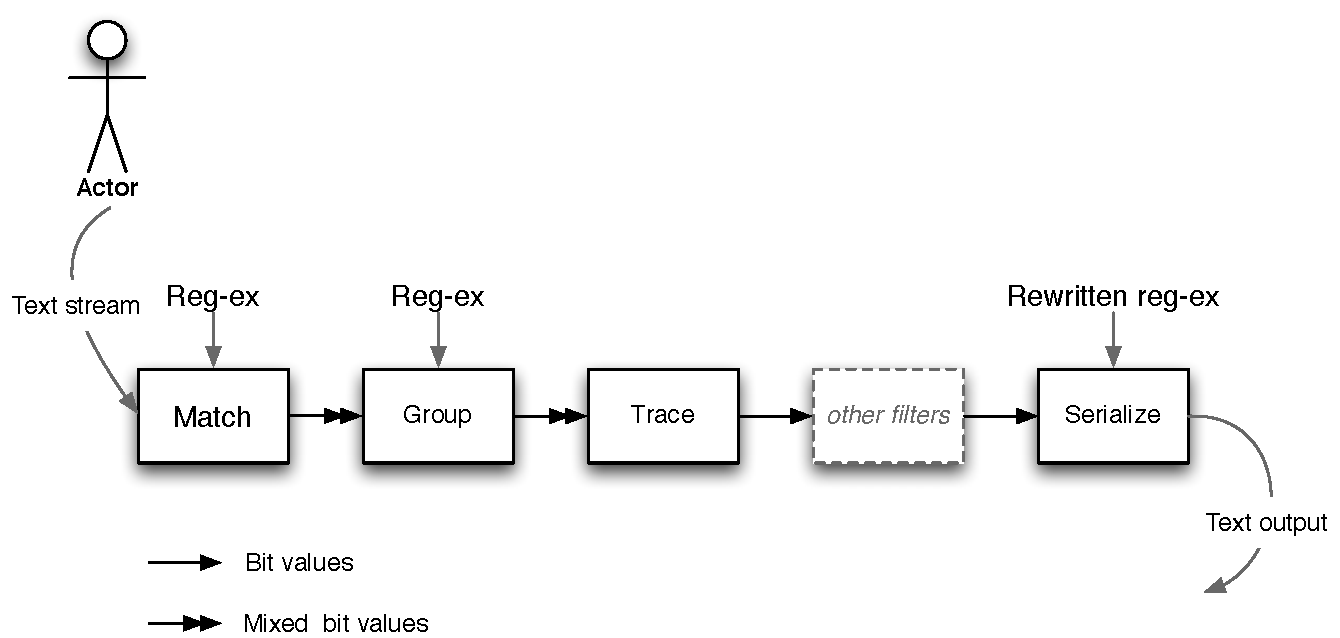
\includegraphics[width=\textwidth]{design/architecture.pdf}
  \caption{Architecture outline}
  \label{fig:architecture}
\end{figure}


%% \todo[inline]{
%% Fleksibel arkitektur (skal tales om sent, det er en implementeringsting):
%%  - hvorfor som unix utility. Plus: nemt at søtte sammen on the fly,
%%  kan nemt serialisiere og transmittere output
%%  - andre alternativer: in-process components. Hvad er drawback: fx
%%  mere bøvlet at sætte sammen on the fly. Hvad er plus: hurtigere
%%  kommunikation mellem komponenter. Reuse af NFA.
 
%% Mixed-bit-values:
%%  Motivation: ?? (kompression?)
%%  Valgmuligheder: alternativer (IKKE IMPLEMENTATION)
%%  Valg
%% }

\subsection{Protocol specification}
\label{sec:protocol_spec}

%\todo[inline]{Introduce the mixed bit-values term.}

In this section we will define a protocol that can communicate
information between our programs. The information consists of the
mixed bit-values generated by the NFA simulator and the filters.

\begin{itemize}
\item The protocol should enable us to recreate paths taken through an
  NFA.
\item The protocol should be one-way. Information can only flow in one
  direction.
\item This protocol is intended to communicate between programs where
  we can expect perfect synchronization and unambiguity. For example
  will it not be necessary to include any error correction. 
%\item Similarly we will not provision for communication between
%  different architectures. 
\item The protocol will be text based, primarily to ease development
  and debugging. It is entirely feasible to later replace this with a
  binary protocol.
\end{itemize}

Our protocol is very compact. The actual implementation may use
different symbols to represent the operators below. We need our
protocol to support the following operators. A description is supplied
for each.

\begin{description}
  \item[\textbar] The end of the channel list is reached and we should
    set the active channel to the first channel. This coincides with
    reading a new character. It is not a strictly necessary operator,
    we can make do with the change channels action. We choose to keep
    a separate action for end of list, because it adds to readability
    and redundancy.
  \item[:] Whenever we change channels we put a :. There may be more
    than one or perhaps even no bits output on a channel for any given
    character from the string
  \item[=] Copying of a channel. One channel is split into two, the
    paths taken through the NFA will be identical up to the point of
    splitting. The newly created channel is put in front of the rest
    of the channels
  \item[0,1] The actual bit values. 
  \item [\textbackslash $a$] The character classes is a special
    case. To later be able to recreate the exact string that we
    matched, we will need to know which character a character class
    matched. To meet this requirement we will output the character we
    matched the character class with in the output. To signal such a
    character is coming we use an escape \textbackslash.
  \item[b] A channel is abandoned with no match
  \item[t] A channel has a match
\end{description}

\begin{example}[Protocol]
  In figure \vref{fig:ex_prot} we have an automaton for regular
  expression \textsf{a*}. When matching this regular expression with
  the string \textsl{aa} we generate some mixed bit-values. This
  example will in detail demonstrate how the mixed bit-values are
  generated.
  \begin{figure}
    \centering
    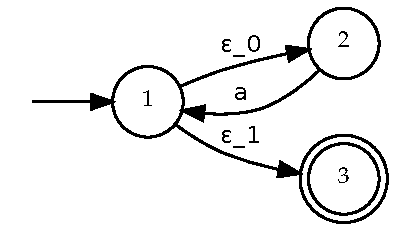
\includegraphics{matching/example_protocol.pdf}
    \caption{Automaton with bitvalues for regular expression
      \texttt{a*}}
    \label{fig:ex_prot}
  \end{figure}
  
  \begin{description}
  
  \item[Initial step:] Initially the start state of the automaton is
    added to the active list. All $\upvarepsilon$-edges are followed
    and the following is output:
    \begin{enumerate}
    \item Node 1 is a split-node, a \texttt{=} is output, and we
      follow the $\upvarepsilon$-edge to node 2 and output a
      \texttt{0}. We can not make any further progress on this
      channel. We output a \texttt{:} and switch to the next channel.

      Output so far: \texttt{=0:}. \\
      List of active channels: $\{2, 1\}$.
    \item The active channel is now in node 1, we follow the
      $\upvarepsilon$-edge from node 1 to 3 and output a
      \texttt{1}. We can not make any further progress on this
      channel. This is the last channel in the channel list, so we
      output a \texttt{|} and reset the active channel.

      Output so far: \texttt{=0:1|}.\\
      List of active channels: $\{2, 3\}$.
    \end{enumerate}

  \item[First \textsl{a} is read]
    \begin{enumerate}
    \item Node 2 has a transition marked \texttt{a}, we follow this
      back to node 1. Node 1 is a split-node, a \texttt{=} is output,
      and we follow the $\upvarepsilon$-edge to node 2 and output a
      \texttt{0}. We can not make any further progress on this
      channel. We output a \texttt{:} and switch to the next channel.

      Output so far: \texttt{=0:1|=0:}. \\
      List of active channels: $\{2, 1, 3\}$.
    \item The active channel is now in node 1, we follow the
      $\upvarepsilon$-edge from node 1 to 3 and output a
      \texttt{1}. We can not make any further progress on this
      channel. We output a \texttt{:} and switch to the next channel.

      Output so far: \texttt{=0:1|=0:1:}. \\
      List of active channels: $\{2, 3, 3\}$.
    \item Node 3 is the accepting node and does not have any
      transitions. We abandon this channel and output a
      \texttt{b}. This is the last channel in the channel list, so we
      output a \texttt{|} and reset the active channel.

      Output so far: \texttt{=0:1|=0:1:b|}. \\
      List of active channels: $\{2, 3\}$.
    \end{enumerate}
  \item[Second \textsl{a} is read] This is the final step.
    \begin{enumerate}
      \item From node 2 we can make a transition on \texttt{a} back to
        node 1. This is a split node, so we output a \texttt{=} and
        transition on the the $\upvarepsilon$-edge to node 2 and
        output a \texttt{0}. We can not do further transitions and
        this is not the accepting node, we abandon this channel and
        output a \texttt{b}. We switch to the next channel and output
        a \texttt{:}.

        Output so far: \texttt{=0:1|=0:1:b|=0b:}. \\
        List of active channels: $\{1, 3\}$.
      \item Node 1 has a $\upvarepsilon$-transition to node 3, we take
        it and output a \texttt{1}. We can not do further transitions
        and since this is the accepting node, we output a
        \texttt{t}. We have one channel left, so we output a
        \texttt{:} and switch.

        Output so far: \texttt{=0:1|=0:1:b|=0b:1t:}. \\
        List of active channels: $\{3\}$.
      \item Node 3 has no available transitions. We abandon this
        channel and output a \texttt{b}.

        Output so far: \texttt{=0:1|=0:1:b|=0b:1t:b}. \\
        List of active channels: $\{\}$.
    \end{enumerate}
  \end{description}
\end{example}

\subsection{Filters}

We have now established that filters are stand-alone programs that
takes input, performs some projection and outputs the result. In this
subsection we will give a more detailed description of the filters
developed for this thesis. 

The filters can be combined to make a whole, naturally some orders of
combining makes more sense than others. For example will it make sense
to have filters removing unnecessary information as early as possible,
to reduce the input data-sizes for downstream filters.

%% \todo[inline]{Better introduction or consider merging with architecture}

%% \todo[inline]{Describe orders of filters}


\subsubsection{The 'match' filter}

\paragraph{Input} Any mixed bit-values or bit-values
\paragraph{Output} A single value indicating match or no match.
\paragraph{}

This is a simple filter. The input is scanned for a \texttt{t} control
character, if present we output a \texttt{t} otherwise we output a
\texttt{b}. In the case of empty input, we will output an error
message, this is because the empty input is most likely due to an
error in the previous programs. To save time on processing, we will
assume the input format is correct.

\begin{example}
The regular expression \textsf{a*} matches the string \textsl{aaa}:
\begin{verbatim}
$ echo -n 'aaa' | ./main 'a*' | ./ismatch 
t
\end{verbatim}
\textsf{a*} does \emph{not} match \textsl{bbb}:
\begin{verbatim}
$ echo -n 'bbb' | ./main  'a*' | ./ismatch 
b
\end{verbatim}
Since we do not check the correctness of the input, the sentence:
``the cake is a lie'' which is clearly not in the correct input format
with regards to the protocol defined section \vref{sec:protocol_spec},
will also produce a positive answer from the filter:
\begin{verbatim}
$ echo -n 'the cake is a lie' | ./ismatch
t
\end{verbatim}

\end{example}

\subsubsection{The 'trace' filter}
\label{sec:desc_materialize}
\paragraph{Input} Mixed bit-values
\paragraph{Output} Bit-values
\paragraph{}

The mixed bit-values is a way of keeping track of multiple paths
through the NFA. This filter will remove all channels from the mixed
bit-values, except the one that has a match. We are using
Thompsons method for matching, so we can be sure there is at most one
channel with a match. 

This will be a non-streaming filter. This problem can not be solved
without in some way storing the mixed bit-values: We need knowledge of
whether or not a channel has a match at the beginning, but we will not
have that knowledge until the end.

\begin{example}
In the previous example we saw that the regular expression \textsf{a*}
matches the string \textsl{aaa}. The NFA for the regular expression is
in figure \vref{fig:ex_prot}, marked with state numbers and
bit-values. This particular match will generate the following mixed
bit-values: \texttt{=0:1|=0:1:b|=0:1:b|=0b:1t:b}. The filter should
then only return the bit-values \texttt{0001}, which represents the
match. The filter should return the empty string if there is no match.
\end{example}


\subsubsection{The 'groupings' filter}
\label{sec:groupings_filter_analysis}
\paragraph{Input} Mixed bit-values
\paragraph{Output} Mixed bit-values for rewritten regular expression
\paragraph{}

This filter facilitates reporting the content of captured groups. The
filter outputs the mixed bit-values associated with the groupings. By
this we mean that all mixed bit-values generated while inside a
captured group should be sent to output and all mixed bit-values
generated outside a group should be thrown away. By throwing away the
unnecessary bit-values we hope to make the mixed bit-values sequence
shorter. This will be an advantage when the time comes to apply the
trace filter, which is non-streaming, described in section
\vref{sec:desc_materialize}.

\begin{example}[Simple groupings filter]
  \label{ex:simple_groupings}
  Here we have a few simple examples of what the groupings filter
  should do. 
  \begin{itemize}
  \item
    For regular expression \textsf{(a\textbar b)} matched with
    \textsl{a} the mixed bit-values are \texttt{=0:1\textbar t:b}. Since
    the whole regular expression is contained in a capturing
    parenthesis, nothing should be thrown away. Output should contain
    \texttt{=0:1\textbar t:b}.
  \item
    For regular expression \textsf{(?:a\textbar b)(c\textbar d)} matched
    with \textsl{ac} the mixed bit-values are
    \texttt{=0:1|=0:1:b|t:b}. This time the first part of the regular
    expression is contained only in a non-capturing parenthesis and the
    associated bit-values should be thrown away. We want to keep only the
    bit-values from the second alternation. Output should contain
    \texttt{=:|=0:1:b|t:b}.
  \end{itemize}
  
  In this example we have only dealt with simple examples. Regular
  expressions containing parenthesis under alternation and repetition,
  e.g. \textsf{(a)\textbar b} and \textsf{(a)*}, require extra care
  and will be discussed later.
\end{example}

The output of the groupings filter can be used to navigate the NFA for
the regular expression altered in a similar manner: Everything not in
a capturing parenthesis is thrown away. From example
\vref{ex:simple_groupings} we have the regular expression
\textsf{(?:a\textbar b)(c\textbar d)}, if we throw away everything not
in a capturing parenthesis we have left \textsf{(c\textbar d)}. Stated
in a more formal manner, we can define our first naive rewriting
function $G'$:

\begin{align}
  G'[[\upvarepsilon]] &= \upvarepsilon \notag\\
  G'[[a]] &= \upvarepsilon \notag\\
  G'[[ [...] ]] &= \upvarepsilon \notag\\
  G'[[r'r_2]] &= G'[[r']]G'[[r_2]] \notag\\
  G'[[r'|r_2]] &= G'[[r']]G'[[r_2]] \notag\\
  G'[[r*]] &= G'[[r]] \notag\\
  G'[[r+]] &= G'[[r]] \notag\\
  G'[[r?]] &= G'[[r]] \notag\\
  G'[[(?:r)]] &= G'[[r]] \label{eq:G1_paren}\\
  G'[[(r)]] &= (r) \notag
\end{align}

\paragraph{Capturing under alternation}
As is seen, $G'$ basically throws away anything not in a capturing
parenthesis. There are however a few problems with this definition, as
hinted earlier. Our first problem is regular expression with a
capturing parenthesis under alternation. When the capturing
parenthesis is under the alternation and we throw away the
alternation, we lose a vital choice: There is no longer a way to
signal whether or not a group participates in a match.
\begin{figure}
  \centering
  \subfigure[\textsf{(a)\textbar (b)}]{
    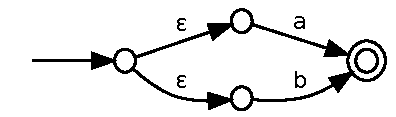
\includegraphics{filters/capturing_under_parenthesis1.pdf}
    \label{fig:capt_paren1}
  }
  \subfigure[\textsf{(a)(b)}]{
    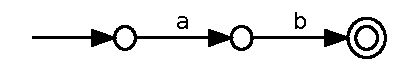
\includegraphics{filters/capturing_under_parenthesis2.pdf}
    \label{fig:capt_paren2}
  }
  \subfigure[\textsf{(?:\textbar (a))(?:\textbar (b))}]{
    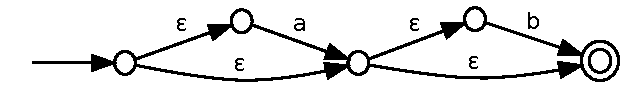
\includegraphics{filters/capturing_under_parenthesis3.pdf}
    \label{fig:capt_paren3}
  }
\caption{Capturing under alternation}
\end{figure}

\begin{example}[Capturing under alternation]
  \label{ex:capturing_under_alternation}
  In matching the regular expression \textsf{(a)\textbar (b)}, see
  figure \vref{fig:capt_paren1} for the NFA, with the string
  \textsl{a} we obtain these mixed bit-values: 
  \begin{center}\texttt{=0:1|t:b}\end{center}
  What these mixed bit-values are saying is that we have 2 channels,
  one that go through \textsf{a} and succeeds and one that go through
  \textsf{b} and fails. The succeeding channel never goes through
  \textsf{b}, the contents of that group is not defined.
  
  Rewriting the regular expression \textsf{(a)\textbar (b)} according
  to $G'$ we have:
  \begin{align*}
    G'[[\text{\textsf{(a)\textbar (b)}}]] &=
    G'[[\text{\textsf{(a)}}]]G'[[\text{\textsf{(b)}}]] \\
    &= \text{\textsf{(a)}}\text{\textsf{(b)}} \\
  \end{align*}
  In this regular expression there is only one way: The one going
  through both the groups. See figure \vref{fig:capt_paren2} for the
  NFA of the expression. This is bad news for our rewriting function
  and our filter, since we need some way of skipping groups: Each
  channel goes through only one group.
\end{example}

In example \ref{ex:capturing_under_alternation} we saw an example of
how undefined groups are not handled. To solve this problem we need
some way of signaling if a group participates in a match or not. We
define a new rewriting function $G''$ it is identical to $G'$ except
for equation \ref{eq:G1_paren} which is changed to:
\begin{align}
    G''[[(r)]] &= (?:|(r)) \notag
\end{align}
This change will enable us to choose which groups participates in a
match. This comes at a cost: Extra bits will have to be added to the
mixed bit-values output and extra alternations to the rewritten
regular expression. 

\begin{example}[continues=ex:capturing_under_alternation]
With the changed equation \ref{eq:G1_paren} we can continue our
example from before. Again we rewrite regular expression
\textsf{(a)\textbar (b)}, this time according to $G''$:
  \begin{align*}
    G''[[\text{\textsf{(a)\textbar (b)}}]] &=
    G''[[\text{\textsf{(a)}}]]G''[[\text{\textsf{(b)}}]] \\
    &= \text{\textsf{(?:\textbar (a))(?:\textbar (b))}} \\
  \end{align*}
  See figure \vref{fig:capt_paren3} for the NFA. As is clear from the
  rewritten regular expression and the NFA, there is now a way around
  the groups. Taking this into account, the output for the groupings
  filter should be: 
  \begin{center}\texttt{=1:01|0t:b}\end{center}
  What these mixed bit-values are saying is that we have two channels,
  one picks the route through \textsf{a}, around \textsf{b} and
  succeeds and the other picks the route around \textsf{a}, through
  \textsf{b} and fails.
\end{example}
As needed, we now have a way of signaling if a particular group is in
a match: Insert a 1 in the mixed bit-values and the group participates
or insert a 0 and it does not. 


\paragraph{Capturing under repetition}
The other problem we hinted at has to do with capturing under
repetition. When using a capturing subpattern, it can match repeatedly
using a quantifier. For example matching \textsf{(.)*} with the string
\textsl{abc}, the first time we apply the \textsf{*} we capture a
\textsl{a} the second time a \textsl{b} and the last time a
\textsl{c}. In such a case we have several options when reporting the
strings that was captured:
\begin{itemize}
\item The first
\item The last, this is the what most backtracking engines like Perl
  do
\item All, this is what a full regular expression engine do
\end{itemize}
Only two of these options are available to a streaming filter: All and
the first. In order to return the last match, we would have to save
the latest match when matching with the quantifier, it is potentially
the last and we can not know until we are done matching with the
quantifier.

Returning the first string that was captured by the quantifier, forces
us to throw away mixed bit-values generated in a capturing
parenthesis. We would only need the mixed bit-values generated by the
first iteration of the quantifier. 

To return all the strings captured by a group, we simply output all
the mixed bit-values generated while in the capturing
parenthesis. However, this causes problems with the rewriting
function. Rewriting \textsf{(.)*} according to $G''$ we have
\textsf{(.)}. This regular expression accepts one single character. In
no way can we make mixed bit-values, fitting this regular expression,
that represent a list of matched strings. Therefore we add the
following equations:
\begin{align*}
  G''[[(r)*]] &= (r)* \\
  G''[[(r)+]] &= (r)+
\end{align*}
We should now also keep the mixed bit-values that glues the iterations
together, even though they are outside the capturing group.




%% \begin{example}[Capturing under repetition]
%%   %% \begin{figure}
%%   %%   \centering
%%   %%   \subfigure[\textsf{(a)*}]{
%%   %%     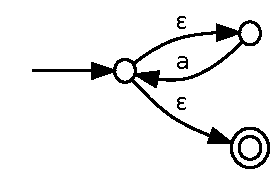
\includegraphics{filters/capt_under_rep1.pdf}
%%   %%     \label{fig:capt_rep1}
%%   %%   }
%%   %%   \subfigure[\textsf{(a)}]{
%%   %%     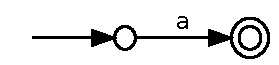
\includegraphics{filters/capt_under_rep2.pdf}
%%   %%     \label{fig:capt_rep2}
%%   %%   }
%%   %%   \caption{Capturing under repetition}
%%   %% \end{figure}

%%   %% In this example we will be matching regular expression
%%   %% \textsf{(a)*}, see figure \vref{fig:capt_rep1} for the NFA, with the
%%   %% string \textsl{aaa}. This match generates the following mixed
%%   %% bit-values:
%%   %% \begin{center}\texttt{=0:1|=0:1:b|=0:1:b|=0b:1t:b}\end{center}

%%   %% Rewriting \textsf{(a)*} according to $G''$ gives us:
%%   %% \begin{align*}
%%   %%   G''[[\text{\textsf{(a)*}}]] &= G''[[\text{\textsf{(a)}}]] \\
%%   %%   &= \text{\textsf{(a)}}
%%   %% \end{align*}
%%   %% See figure \vref{fig:capt_rep2} for the NFA.

%%   %% This rewrite works if we are only interested in one 

%%   By matching
%% \end{example}


%% To return all we need to make some changes to the rewriting function,
%% we add the following equations:
%% \begin{align*}
%%   G''[[(r)*]] &= (r)* \\
%%   G''[[(r)+]] &= (r)+
%% \end{align*}


%% We should not just throw away everything

%% If we choose to return all, all we need to do is add equations to the
%% rewriting function:
%% \begin{align*}
%%   G''[[(r)*]] &= (r)* \\
%%   G''[[(r)+]] &= (r)+
%% \end{align*}



%% Returning all would be the easier solution. We need to be careful when
%% rewriting the regular expression however. With the output from the
%% groupings filter we should be able to navigate the NFA for the
%% rewritten regular expression.


%% Returning all would be the easiest solution, this would however
%% require a change in the rewriting function. We add the equations:
%% \begin{align*}
%%   G''[[(r)*]] &= (r)* \\
%%   G''[[(r)+]] &= (r)+
%% \end{align*}


%% %% Returning all of the strings that were captured is by far the easiest,
%% %% no extra work is required. On the other hand if we only want to return
%% %% the first of the matches, we need to know whether or not to return a
%% %% particular match, that is if this is the first time we match with the
%% %% quantifier or not. If we alter the way we construct the NFA, we can
%% %% achieve this. 





%% \todo{Hvad den blippen er det nu for en løsning jeg har på det
%%   problemos}



We are now ready to present the final rewriting function: Definition
\vref{def:G}.
\begin{definition}[The groupings filter rewriting function]
  \label{def:G}
  For regular expressions $r$, $r_1$, $r_2$, defined over alphabet
  $\Sigma$, and $a$, any character from $\Sigma$, let $G$ be defined by:
  \begin{align*}
    G[[\upvarepsilon]] &= \upvarepsilon \\
    G[[a]] &= \upvarepsilon \\
    G[[ [...] ]] &= \upvarepsilon \\
    G[[r_1r_2]] &= G[[r_1]]G[[r_2]] \\
    G[[r_1|r_2]] &= G[[r_1]]G[[r_2]] \\
    G[[r*]] &= G[[r]] \\
    G[[r+]] &= G[[r]] \\
    G[[r?]] &= G[[r]] \\
    G[[(?:r)]] &= G[[r]] \\
    G[[(r)]] &= (?:|(E)) \\
    G[[(r)*]] &= (?:|(r)*) \\
    G[[(r)+]] &= (?:|(r)+) \\
  \end{align*}
\end{definition}
\begin{example}
  Here follows a few examples of how the groupings filter rewriting
  function, $G$, works.
  \begin{align*}
    G[[\mathsf{(a)|b}]] &= G[[\mathsf{(a)}]]G[[\mathsf{b}]]\\
    &= \mathsf{(?:(a))} \upvarepsilon\\
    &= \mathsf{(?:(a))}
  \end{align*}

  \begin{align*}
    G[[\mathsf{((cup)cake)}]] &= \mathsf{(?:|((cup)cake))}
  \end{align*}

  \begin{align*}
    G[[\mathsf{(a|b)*}]] &= \mathsf{(a|b)*}
  \end{align*}
\end{example}


